%中南大学硕士学位论文模板(按学校格式要求自制,非官方发布) 
%时间:2020年6月25日
%作者:钟乙源 zhongyiyuan@csu.edu.cn
%导师:任政勇
%单位:地球科学与信息物理学院
%%%%%%%%%%%%%%%%%%%%%%%%%%%%%%%%%%%%%%%%%%%%%%%%%%%%%%
% Copyright © 2020 钟乙源
% 未经作者允许,不得以本模板用于任意形式的盈利性活动。
% 作者对使用本模板造成的直接或间接损失不负任何责任。
%%%%%%%%%%%%%%%%%%%%%%%%%%%%%%%%%%%%%%%%%%%%%%%%%%%%%%

\documentclass[a4paper,12pt,twoside]{report}
%% 文档类型使用report或者book都可以,但是不能用article,因为article中没有chapter
%% a4paper 表示纸张幅面宽210mmX高297mm
%% openright 表示新的一章从右页开始,openany表示每一章从左页(即双面时的背面)或者右页(即双面打印时的正面)开始都可以
%% twoside 表示区分左右页

%\usepackage[no-math]{fontspec}
\usepackage{fontspec}
%%%%%%%%%%%公式配置%%%%%%%%%%%%%%
\usepackage[intlimits,sumlimits]{amsmath}
%\usepackage{txfonts}
%\usepackage{nccmath}
\usepackage{amssymb}
\usepackage{amsbsy}
\usepackage{bm}
%\usepackage{wasysym}

%\usepackage{unicode-math}
\usepackage{amsfonts}
\usepackage{mathptmx}
\usepackage{esint}%The package esint.sty allows you to use new integrals symbols.

%%公式编号方式
\renewcommand{\theequation}{\thechapter-\arabic{equation}}%%公式编号形式为(章-公式号),如(1-1)

%中文字体宏包ctex
%默认小四号字体,采用半角标点
\usepackage{xeCJK}
\xeCJKsetup{AutoFakeBold=2.5}
\usepackage[zihao=-4,space,heading,scheme=chinese,punct=banjiao]{ctex}


%\usepackage{mathptmx}
\setCJKfamilyfont{hwxw}{华文新魏}%使用windows中的华文新魏字体
\newcommand{\xinwei}{\CJKfamily{hwxw}}
\setmainfont{Times New Roman}%设置英文字体为Times New Roman

%%%%版式%%%%%%%
%用A4规格输出,打印区面积为240mm×146mm(包括篇眉),页脚距底端距离为 1.75 厘米,页眉至顶端距离为 1.5 厘米
%A4 297mmX210mm
%见https://www.jianshu.com/p/0719795278eb
%\usepackage[includehead,left=32mm,right=32mm,top=27mm,bottom=30mm]{geometry}textheight=240mm
\usepackage[includehead,left=32mm,right=32mm,textheight=240mm,headsep=5mm,bottom=27mm,footskip=9.5mm]{geometry}

%设置页边距的命令要在设置页眉的命令之前
\usepackage{layout}
\usepackage{paralist}
\usepackage{fancyhdr}
\pagestyle{fancy}%设置页眉
%\fancyhead{}
%\fancyhead[L]{}
%\fancyhead[R]{
%}
\usepackage[dvipsnames]{xcolor}
\renewcommand{\headrule}{\color{lightgray}\hrule width\headwidth height0.9pt}
%\renewcommand{\headrulewidth}{3pt}

\usepackage{algorithm}
\usepackage{algorithmicx}
\makeatletter
\floatname{algorithm}{\zihao{-4} 算法}

\usepackage{algpseudocode} 

\renewcommand{\algorithmicrequire}{\textbf{}}

\usepackage{array}%制作表格宏包
\newcommand{\PreserveBackslash}[1]{\let\temp=\\#1\let\\=\temp}
\newcolumntype{C}[1]{>{\PreserveBackslash\centering}m{#1}}
\newcolumntype{R}[1]{>{\PreserveBackslash\raggedleft}m{#1}}
\newcolumntype{L}[1]{>{\PreserveBackslash\raggedright}m{#1}}
\usepackage{multirow}
\usepackage{booktabs}

%%%%%%%%%插图宏包
\usepackage{graphicx}
\usepackage{subfig}
\usepackage{caption}
\usepackage{float}
\DeclareCaptionLabelSeparator{figurelabelset}{\hspace{1em}} 
\DeclareCaptionFont{figurefont}{\heiti\zihao{5}}
\DeclareCaptionFont{figurelabelfont}{\kaishu\zihao{5}}
\DeclareCaptionFont{figuretextfont}{\kaishu\zihao{5}}
\captionsetup{
    labelsep=figurelabelset,
    format=hang,
    %justification=centerfirst
	labelfont=figurelabelfont,
	textfont=figuretextfont,
    belowskip=-0.5ex
}

%调节图表名上下的间距
\newcommand{\topcaption}{%
	\setlength{\abovecaptionskip}{3.5pt}%
	\setlength{\belowcaptionskip}{-5pt}%
	\caption}
\setlength{\abovecaptionskip}{5pt}%
\setlength{\belowcaptionskip}{-7.5pt}%


\renewcommand{\thefigure}{\thechapter-\arabic{figure}}
\renewcommand{\thetable}{\thechapter-\arabic{table}}

\usepackage{lastpage}


%各级标题格式设置
\ctexset{
    chapter={
        number=\arabic{chapter},
        format=\bfseries\zihao{3}\centering,
%        name={,},
        nameformat=\zihao{3}\heiti,
        titleformat={\zihao{3}\heiti},
        afterskip=15pt,
        beforeskip=-5pt,
        pagestyle={fancy}
    }
}
\ctexset{
    section={
        format=\mdseries\zihao{-4}\heiti,
%        indent=\parindent,
        beforeskip=0.8ex,
        afterskip=0.5ex,
    }
}
\ctexset{
    subsection={
        format=\mdseries\zihao{-4},
%        indent=\parindent,
        beforeskip=0.8ex,
        afterskip=0.5ex,
    }
}


%GBT参考文献https://gitee.com/walkeraguo/gbt7714-bibtex-style
\usepackage[sort&compress]{gbt7714}
\bibliographystyle{gbt7714-numerical}
\usepackage{natbib}
\setlength{\bibsep}{3pt}
\usepackage[colorlinks=true,breaklinks=true]{hyperref}
\hypersetup{
  linkcolor=black,
  citecolor=blue,
  bookmarksnumbered=true,
}

\renewcommand{\thefootnote}{\roman{footnote}}
\usepackage{titletoc}


\titlecontents{chapter}[0pt]{\heiti}
{\contentspush{\thecontentslabel\hspace*{0.5em}}}
{}{\titlerule*[5pt]{.}\contentspage}

\titlecontents{section}[2em]{}
{\contentspush{\thecontentslabel\hspace*{0.5em}}}
{}{\titlerule*[5pt]{.}\contentspage}

\titlecontents{subsection}[4em]{}
{\contentspush{\thecontentslabel\hspace*{0.5em}}}
{}{\titlerule*[5pt]{.}\contentspage}
\makeatletter
\renewcommand\@dotsep{0.5}%指引线中相邻点的距离
\renewcommand{\@pnumwidth}{0.5em}
\makeatother

\usepackage{wallpaper}
\usepackage[titletoc,title]{appendix}
\usepackage{lipsum}

%题目
\newcommand{\mytitle}{自制中南大学硕士论文\LaTeX 模板}
%英文题目
\newcommand{\myEnlishTitle}{A \LaTeX  ~template for master thesis submitted to Central South University}
%作者姓名
\newcommand{\myName}{钟乙源}
%学科专业
\newcommand{\major}{地质资源与地质工程}
%学科方向
\newcommand{\discipline}{地球探测与信息技术}
%研究方向,学校提供的的格式中有“学科方向”和“研究方向”这两个,不知道什么区别
\newcommand{\researchTopic}{地球探测与信息技术}
%学院
\newcommand{\school}{地球科学与信息物理学院}
%导师
\newcommand{\mySupervisor}{任政勇 教授}
%副导师
\newcommand{\myAssociateSupervisor}{汤井田 教授}
%中图分类号,网上搜
\newcommand{\zhongtu}{P631.1}
%UDC,网上搜
\newcommand{\UDC}{550}
\newcommand{\defendYear}{2020}
\newcommand{\defendMonth}{6}
\begin{document}
    \songti
    
    \linespread{1.56}\selectfont%正文前采用宽一点的行距,后面正文开始前再改成学校规定的20pt行距,不然太难看
    
    %%cover.tex文件中包含:封面、扉页
    %封面
\pdfbookmark{球坐标系下重力数据的约束自适应反演}{title}
\linespread{1.56}\selectfont%正文前采用宽一点的行距,后面正文开始前再改成学校规定的20pt行距,不然太难看
\begin{titlepage}
	\thispagestyle{empty}
	
%	\ThisTileWallPaper{\paperwidth}{\paperheight}{figures/titlepage.jpg}
	\begin{center}
		\vspace*{6em}
		{\heiti \zihao{-2} \bfseries 硕士学位论文}\par
		\vspace{3.5em}
		{\heiti \zihao{2}\bfseries \mytitle}\\
		\vspace{2em}
		{\zihao{-2}\bfseries\myEnlishTitle}\\
		\vspace{6em}
		{\zihao{3}
			\begin{tabular}{>{\songti}r >{\songti}l}			
				\bfseries 学 科 专 业\quad               &\bfseries \major  \\[19pt]
				\bfseries 学 科 方 向\quad               &\bfseries \discipline  \\[19pt]
				\bfseries 作 者 姓 名\quad     &\bfseries \myName  \\ [19pt]
				\bfseries 指 导 教 师\quad               &\bfseries \mySupervisor\\ [19pt]
			\end{tabular}
		}
		
		\zihao{3}
		\vspace{5em}
		{\songti \zihao{-3} 中 南 大 学\\ 2020年6月}	
	\end{center}
\end{titlepage}
\thispagestyle{empty}
\begin{center}
	\newlength{\ztfl}\settowidth{\ztfl}{\zihao{4} \makebox[65pt][s]{中图分类号} \uline{\makebox[5em][c]{}}}
	\begin{minipage}[t]{\ztfl}
		\zihao{4}
		{\songti \makebox[65pt][s]{中图分类号} \uline{\makebox[5em][c]{\zhongtu}}}\\
		{\makebox[65pt][s]{UDC} \uline{\makebox[5em][c]{\UDC}}}
	\end{minipage}\hfill
	\newlength{\SchoolCodeLength}\settowidth{\SchoolCodeLength}{\zihao{4} 学位类别~~~\quad 学术学位}
	\begin{minipage}[t]{\SchoolCodeLength}
		\zihao{4}
		{\songti 学校代码\uline{\quad 10533~~~~\quad}}\\
		{\songti 学位类别\uline{\quad 学术学位~~}}
	\end{minipage}
	\vspace{5em}\\
	{\heiti \zihao{-2}\bfseries 硕士学位论文}\par
	\vspace{2em}
	{\heiti \zihao{2}\bfseries \mytitle}\\
	\vspace{1em}
	{\zihao{-2}\bfseries\myEnlishTitle}
	\vspace{3em}
\end{center}
\begin{center}
	\zihao{3}
	\begin{tabular}{>{\songti}r >{\songti}l}
		% after \\: \hline or \cline{col1-col2} \cline{col3-col4} ...
		作 者 姓 名:\quad     &\myName  \\
		学 科 专 业:\quad               &\major  \\
		学 科 方 向:\quad               &\discipline  \\
		研 究 方 向:\quad               &\researchTopic  \\
		二级培养单位:\quad    & \school \\
		指 导 教 师:\quad               &\mySupervisor\\
		副指导教师:\quad               &\myAssociateSupervisor\\
	\end{tabular}\\
	\vspace{3em}
	
	{\songti \zihao{-3} 论文答辩日期:\uline{\makebox[8.5em][c]{}}}
	\hfill
	{\songti \zihao{-3} 答辩委员会主席:\uline{\makebox[5em][c]{}}}
	
	\vspace{3em}
	{\songti \zihao{-3} 中 南 大 学\\ \defendYear 年\defendMonth 月}        
\end{center}
\newpage \thispagestyle{empty}~
    %%copyright.tex文件中包含“学位论文原创性声明”和“版权使用授权书”
    \clearpage
\thispagestyle{empty}
\begin{center}
	\zihao{2}\xinwei 学位论文原创性声明
\end{center}
\zihao{4}

本人郑重声明,所呈交的学位论文是本人在指导教师指导下进行的研究工作及取得的研究成果。尽我所知,除了论文中特别加以标注和致谢的地方外,论文中不包含其他人已经发表或撰写过的研究成果,也不包含为获得中南大学或其他教育机构的学位或证书而使用过的材料。与我共同工作的同志对本研究所作的贡献均已在论文中作了明确的说明。

申请学位论文与资料若有不实之处,本人承担一切相关责任。
\vspace{3em}

\hfill 
作者签名:\uline{\makebox[3cm][c]{}}\quad\quad\quad 日期:\uline{\makebox[1.5cm][c]{}}年\uline{\makebox[1cm][c]{}}月\uline{\makebox[1cm][c]{}}日
\vspace{5em}
\begin{center}
	\zihao{2}\xinwei 学位论文版权使用授权书
\end{center}

本学位论文作者和指导教师完全了解中南大学有关保留、使用学位论文的规定:即学校有权保留并向国家有关部门或机构送交学位论文的复印件和电子版;本人允许本学位论文被查阅和借阅;学校可以将本学位论文的全部或部分内容编入有关数据库进行检索,可以采用复印、缩印或其它手段保存和汇编本学位论文。

保密论文待解密后适应本声明。
\vspace{2em}

\noindent
{\songti \zihao{-3}  作者签名:\uline{\makebox[6em][c]{}}}\hfill
{\songti \zihao{-3}  指导老师签名:\uline{\makebox[6em][c]{}}\quad}\\[1em]
{\songti \zihao{-3}  日期:\uline{\makebox[1.5cm][c]{}}年\uline{\makebox[1cm][c]{}}月\uline{\makebox[1cm][c]{}}日}\hfill
{\songti \zihao{-3}  日期:\uline{\makebox[1.5cm][c]{}}年\uline{\makebox[1cm][c]{}}月\uline{\makebox[1cm][c]{}}日}
\vspace{3em}
\newpage \thispagestyle{empty}~
    
    \fancyhead{}
    \pagenumbering{Roman}
    \fancyhead[L]{} 
    %%abstract.tex文件中包含中英文摘要

    %中文摘要
\newpage
%页眉
\fancyhead[L,C,R]{}
\renewcommand{\headrule}{\color{lightgray}\hrule width\headwidth height0.0pt}
%居中打印论文题名(三号黑体)
%\begin{center}
%	\heiti
%	%\fontsize{16.06pt}{20pt}\selectfont%三号字体
%	\zihao{3}
%	\bfseries
%	\mytitle
%\end{center}
\chapter*{\mytitle}
%\addcontentsline{toc}{chapter}{摘要}

\zihao{4}\setlength{\baselineskip}{20pt}

\noindent{\heiti 摘要}:滚滚长江东逝水,浪花淘尽英雄。是非成败转头空。青山依旧在,几度夕阳红。

白发渔樵江渚上,惯看秋月春风。一壶浊酒喜相逢。古今多少事,都付笑谈中。\\
\\
图85幅,表6个,参考文献104篇\\\\
\noindent{\heiti \bfseries 关键词:} 长江;浊酒;笑谈;中南大学;\LaTeXe 模板\\
\noindent{\heiti \bfseries 分类号:} \zhongtu
%英文摘要


\vspace*{1ex}
%\layout
%\begin{center}
%	%\fontsize{18.07}{18.07}\selectfont
%	\zihao{3}\textbf{\myEnlishTitle}
%\end{center}
\chapter*{\myEnlishTitle}
%\addcontentsline{toc}{chapter}{Abstract}

\zihao{4}\setlength{\baselineskip}{20pt}
\noindent\textbf{Abstract}: Lorem ipsum dolor sit amet, consectetuer adipiscing elit. Utpurus elit, vestibulum ut, placerat ac, adipiscing vitae, felis. Curabitur	dictum gravida mauris. Nam arcu libero, nonummy eget, consectetuer id,	vulputate a, magna. Donec

Nam dui ligula, fringilla a, euismod sodales, sollicitudin vel, wisi. Morbi auctor lorem non justo. Nam lacus libero, pretium at, lobortis vi­tae, ultricies et, tellus. Donec aliquet, tortor sed accumsan bibendum, eratligula aliquet magna, vitae ornare odio metus a mi. Morbi ac orci et nislhendrerit mollis. Suspendisse ut massa.\\

\noindent\textbf{keywords:} \LaTeX; template\\
\noindent\textbf{Classification:} \zhongtu

\zihao{-4}%字号改回小四



    %目录设置
%\fancyhead[R]{\slshape 目录}
%\fancyhead[L]{} 
%\ctexset{chapter/format=\zihao{3}\centering}
\pdfbookmark{目录}{contents}
\fancyhead[L,C,R]{}
\renewcommand{\contentsname}{\heiti \zihao{3} 目\quad 录}
\tableofcontents

%\ctexset{chapter/format=\zihao{3}}
    \hypersetup{linkcolor=red}
    


	%%正文页眉设置
	\fancyhead[EL,OR]{\songti\zihao{5} \leftmark}%
	\fancyhead[ER,OL]{\songti\zihao{5} 中南大学硕士学位论文}
	\renewcommand{\headrule}{\color{black}\hrule width\headwidth height0.9pt}
	
	%%正文内容
	%正文行距20pt
	\zihao{-4}
	\setlength{\baselineskip}{20pt}
	
	\pagenumbering{arabic}
%	\fancyfoot[C]{\zihao{-5} 第\thepage 页\quad 共\pageref*{LastPage} 页}
    \chapter{绪论}
\section{使用方法}
\subsection{编译工具配置}
需要使用texlive 2020以上版本。如果用其他低版本的texlive,则需要将dissertation.tex第29行\verb|\xeCJKsetup{AutoFakeBold=2.5}|注释掉,否则会导致生成的pdf无法正常复制,影响查重。

\subsection{编译}
第一次编译需要先编译dissertation.tex文件。

\subsection{内容}
将dissertation.tex中的标题等信息替换成自己的论文信息,摘要在abstract.tex中修改,正文在chapter1.tex、chapter2.tex、chapter3.tex、chapter4.tex、chapter5.tex等文件修改。

\subsection{参考文献}
在bibfile.bib文件里面添加参考文献信息,参考文献信息可以通过百度学术、bing学术、google scholar直接导出成bib文件所需格式。

\section{参考文献引用}
\subsection{上标引用}
使用\verb|\cite{词条名}|进行引用,如\cite{hofmann2006physical}......

\subsection{作者名引用}
使用\verb|\citet{词条名}|进行引用,如\citet{blakely1996potential}做了......

\section{110分钟了解\LaTeXe}
\href{https://mirrors.tuna.tsinghua.edu.cn/CTAN/info/lshort/chinese/lshort-zh-cn.pdf}{https://mirrors.tuna.tsinghua.edu.cn/CTAN/info/lshort/chinese/lshort-zh-cn.pdf}

\section{声明}
本模板版权归作者所有,任何人可以免费使用和转发本模板,无需通知作者。未经作者允许,任何人或组织不得将本模板用于任意形式的盈利性活动,否则追究一切责任。
作者对使用本模板造成的直接或间接损失不负任何责任。

    \chapter{公式}

行内公式的书写格式为\${\kaishu 公式}\$,例如$\mathbf{F}=m\mathbf{a}$。

行间公式需要放在equation环境中,格式为
\begin{verbatim}
\begin{equation}
公式
\end{equation}
\end{verbatim}

例如,
\begin{equation}
\oint_{\Gamma}\mathbf{H}\cdot d\mathbf{l}=\iint_\Omega(\mathbf{J}+\frac{d\mathbf{D}}{dt})\cdot d\mathbf{S}
\end{equation}

多行公式例子如下
\begin{equation}
\begin{split}
a=&b+c+d+e+f+g+h+i\\
=&\frac{x^2+y^{1/2}}{x^2+y^2}\\
=&\sum_{i=0}^{N}x_i^2
\end{split}
\end{equation}

    \chapter{插图}
如图\ref{fig:csu}所示

\begin{figure}[H]
	\centering
	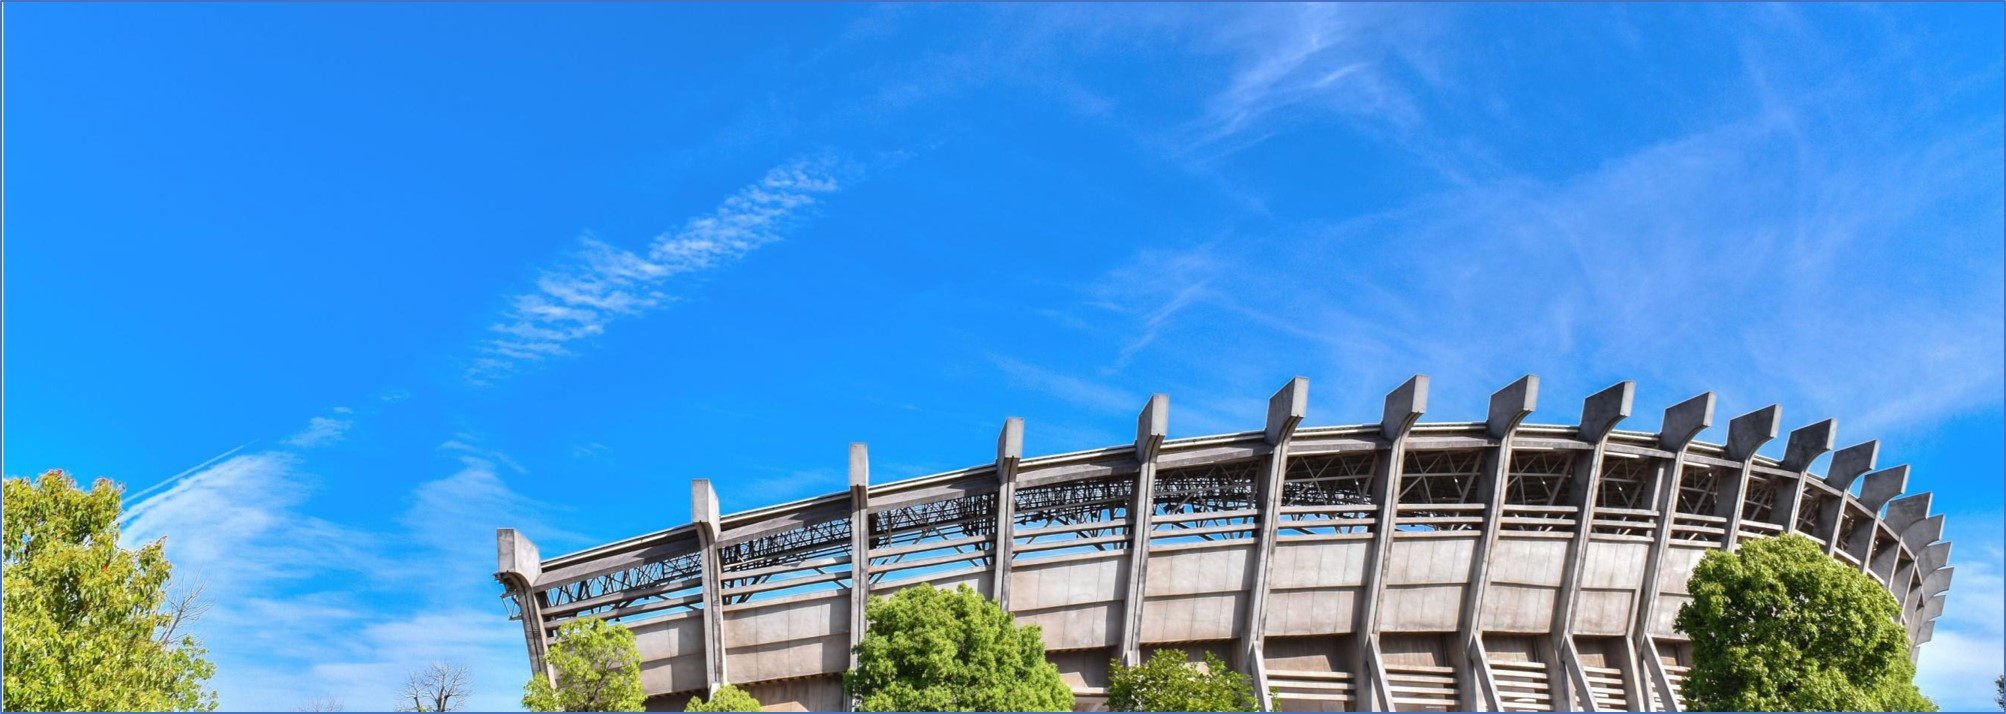
\includegraphics[width=0.8\linewidth]{figures/csu}
	\caption{中南大学}
	\label{fig:csu}%标签,以备交叉引用
\end{figure}
    \chapter{xxx}
    \chapter{结论与建议}
对文章进行总结,如简述本文做了哪些工作,有哪些创新,从研究内容中得出了什么结论,还有对文章的局限性/不足进行阐述,为读者提供建议参考。


    %\include{chapter6}
    %\chapter*{附录}
%\addcontentsline{toc}{chapter}{附录}
\makeatletter
\@addtoreset{equation}{chapter}
\makeatother
\renewcommand{\theequation}{\thechapter-\arabic{equation}}
\numberwithin{table}{chapter}
\numberwithin{figure}{chapter}
\renewcommand{\thefigure}{\thechapter-\arabic{figure}}
\renewcommand{\thetable}{\thechapter-\arabic{table}}
\appendix
\chapter{abcd}\label{cha:appendix1}
\begin{equation}
1+1=2
\end{equation}
    %\zihao{-5}
%\kaishu
%\renewcommand{\bibsetup}{\linespread{1.5}\selectfont}
%\setlength\bibitemsep{0pt}
%\defbibheading{bibliography}{%
%\zihao{3}%
%\heiti%
%\chapter*{#1}%
%\addcontentsline{toc}{chapter}{#1}}
%\renewcommand{\bibfont}{\fontsize{9.03}{9.03}\selectfont}
%\printbibliography[title={参考文献},heading=bibliography]

\bibliography{bibfile.bib}
\addcontentsline{toc}{chapter}{参考文献}
    
    \ctexset{
    	chapter={
    		name={,},
    		aftername=\hspace*{0pt},
    		number={},
    		format=\centering
    	}
    }
%	\fancyhead[EL,OR]{\songti\zihao{5} \leftmark}%
    
\chapter*{攻读学位期间主要成果}
\chaptermark{攻读学位期间主要成果}
\addcontentsline{toc}{chapter}{攻读学位期间主要成果}
\section*{已发表期刊论文}
\begin{enumerate}[{[}1{]}]
	\item a
	\item b
	\item c
\end{enumerate}


\section*{会议论文}





    \chapter*{致\quad 谢}
%\section{xxx}
\chaptermark{致谢}
\addcontentsline{toc}{chapter}{致谢}


谢谢







    %\bibliographystyle{plain}%
    %\bibliography{bibfile}

\end{document}
